\chapter{使用 tikz 绘制示意图}

\begin{texcode}
\usetikzlibrary {arrows.meta,graphs,shapes.misc}
\tikz [>={Stealth[round]}, black!50, text=black, thick,
      every new ->/.style = {shorten >=1pt},
      graphs/every graph/.style = {edges=rounded corners},
      skip loop/.style = {to path={-- ++(0,#1) -| (\tikztotarget)}},
      hv path/.style = {to path={-| (\tikztotarget)}},
      vh path/.style = {to path={|- (\tikztotarget)}},
      nonterminal/.style = {
        rectangle, minimum size=6mm, very thick, draw=red!50!black!50, top color=white,
        bottom color=red!50!black!20, font=\itshape, text height=1.5ex,text depth=.25ex},
      terminal/.style = {
        rounded rectangle,  minimum size=6mm, very thick, draw=black!50, top color=white,
        bottom color=black!20, font=\ttfamily, text height=1.5ex, text depth=.25ex},
      shape = coordinate
      ]
  \graph [grow right sep, branch down=7mm, simple] {
    / -> unsigned integer[nonterminal] -- p1 -> "." [terminal] -- p2 -> digit[terminal] --
    p3 -- p4 -- p5 -> E[terminal] -- q1 ->[vh path]
    {[nodes={yshift=7mm}]
      "+"[terminal], q2, "-"[terminal]
    } -> [hv path]
    q3 -- /unsigned integer [nonterminal] -- p6 -> /;

    p1 ->[skip loop=5mm]   p4;
    p3 ->[skip loop=-5mm]  p2;
    p5 ->[skip loop=-11mm] p6;

    q1 -- q2 -- q3;  % make these edges plain
  };
\end{texcode}

\inputminted{latex}{examples/tikz/diagrams/android-activity-lifecycle.tex}

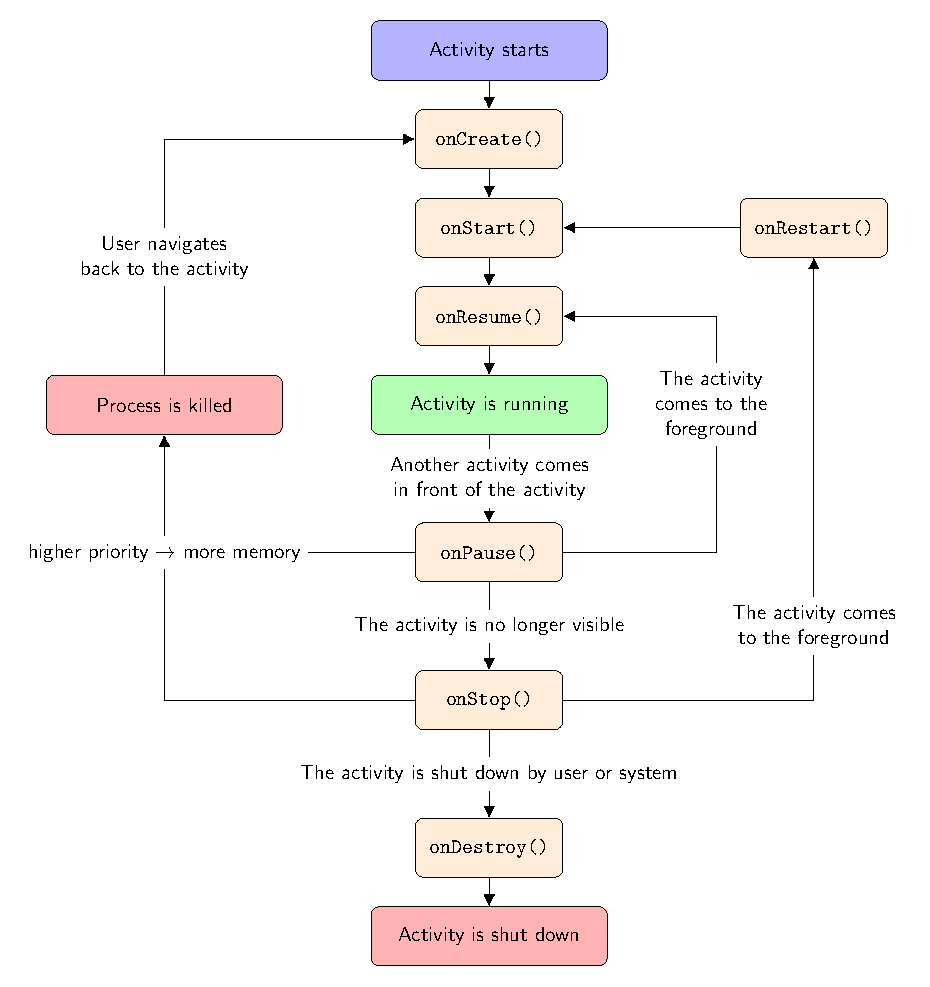
\includegraphics[scale=0.85]{examples/tikz/diagrams/android-activity-lifecycle.pdf}